\capitulo{5}{Aspectos importantes del desarrollo del proyecto}

En este capítulo se describen los aspectos principales del desarrollo del sistema. La solución se ha organizado en torno a dos complementos independientes para Blender: un primer \textit{add-on}, denominado \textit{Data Logger 3D}, encargado de la captura de datos durante la sesión de modelado, y un segundo \textit{add-on}, orientado al análisis, cálculo de métricas y visualización de resultados. Esta separación permite distinguir con claridad la fase de adquisición de datos y la fase de explotación analítica~\cite{parnas1972criteria,pressman2005}.

\section{Planteamiento general del desarrollo}

El desarrollo se llevó a cabo mediante una aproximación iterativa. En primer lugar, se comprobó la viabilidad de monitorizar el estado de la escena mediante la API \texttt{bpy}~\cite{blenderapi}, prestando atención a la captura de transformaciones, cambios de modo, modificaciones topológicas y operaciones relevantes del usuario.

Una vez validada la captura, se definió un formato de persistencia basado en CSV. Esta decisión permitió almacenar los registros de forma estructurada, inspeccionable y reutilizable por el módulo de análisis~\cite{mckinney2022python}. Posteriormente, el trabajo se centró en el cálculo de métricas temporales, espaciales, geométricas y operacionales, así como en la generación de visualizaciones que facilitaran la interpretación de las sesiones registradas~\cite{munzner2014visualization}.

La Figura~\ref{fig:Flujo} resume el flujo general del sistema, desde la interacción del usuario hasta la obtención de resultados analíticos.

\begin{figure}[H]
    \centering
    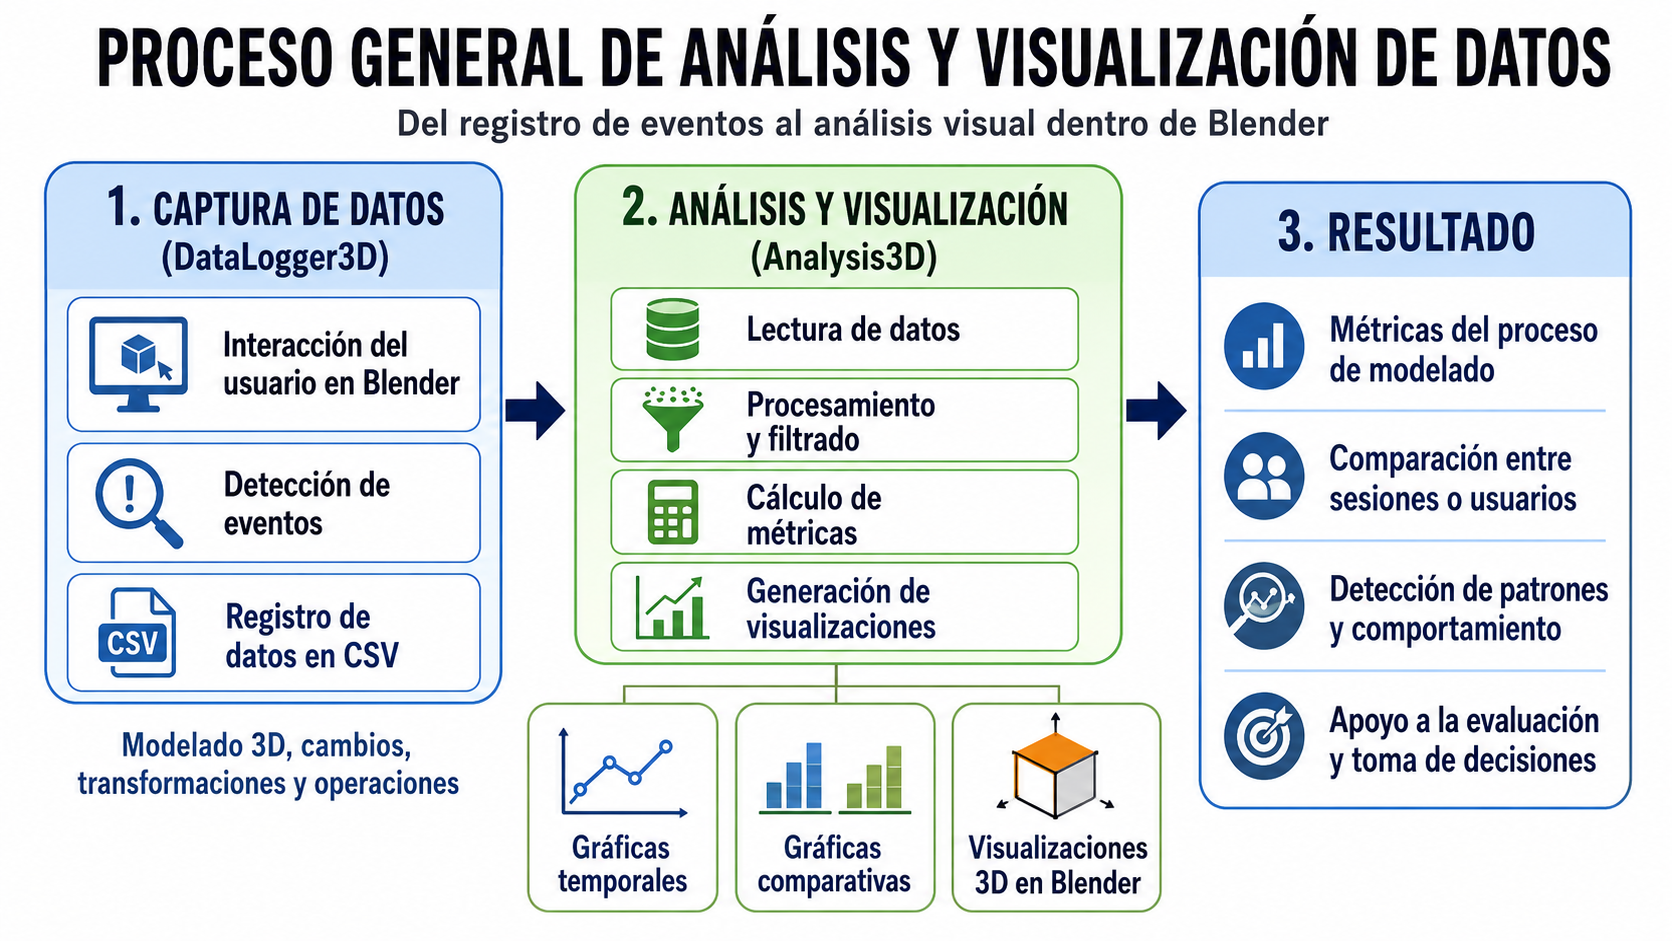
\includegraphics[width=\textwidth, height=0.62\textheight, keepaspectratio]{diagramas/flujo2.png}
    \caption{Flujo general de análisis y visualización de datos de la plataforma.}
    \label{fig:Flujo}
    {\footnotesize \textit{Nota. Figura elaborada por la autora con asistencia de ChatGPT.}}
\end{figure}

\section{Arquitectura general del sistema}

La arquitectura del sistema se basa en una división modular entre captura y análisis. El complemento de captura registra la actividad producida durante el modelado y genera un archivo CSV. El complemento de análisis lee dicho archivo, valida su contenido, calcula métricas y produce resultados visuales y estadísticos.

Esta separación reduce el acoplamiento entre componentes, permite analizar sesiones una vez finalizada la captura y facilita la comparación entre distintos registros. La Figura~\ref{fig:architecture_system} muestra la estructura general de comunicación entre los módulos.

\begin{figure}[H]
    \centering
    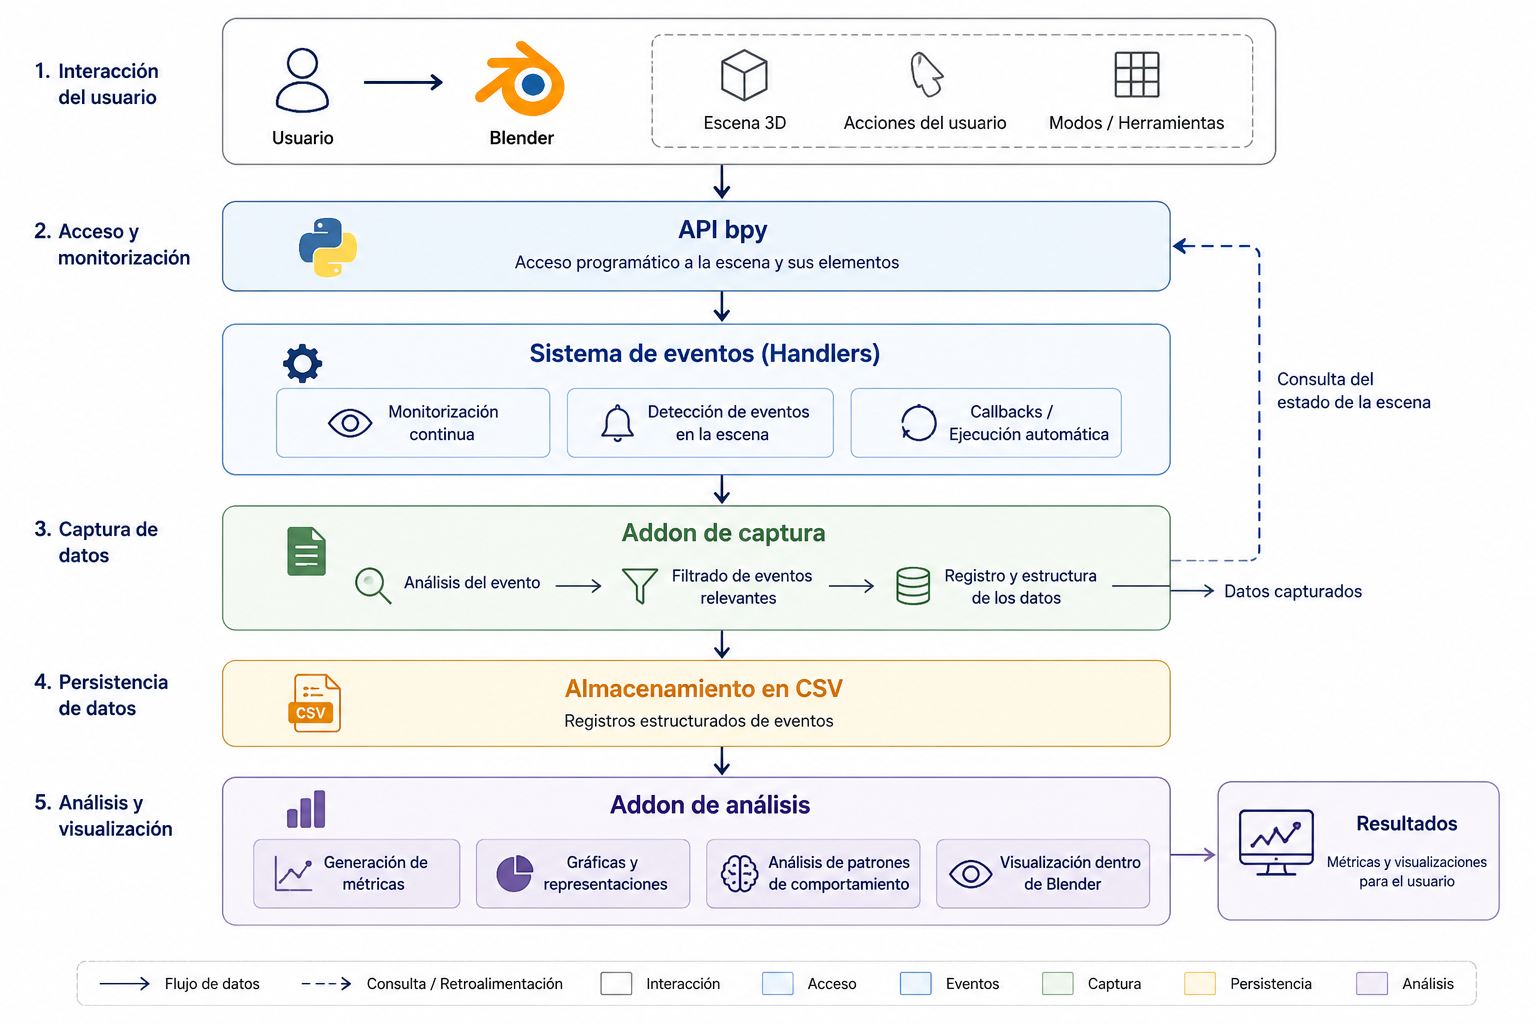
\includegraphics[width=0.95\textwidth]{diagramas/arquitecturaV2.png}
    \caption{Arquitectura general del sistema desarrollado y flujo de comunicación por ficheros.}
    \label{fig:architecture_system}
    {\footnotesize \textit{Nota. Figura elaborada por la autora con asistencia de ChatGPT.}}
\end{figure}

\begin{table}[H]
\centering
\small
\begin{tabularx}{\textwidth}{p{0.28\textwidth}X}
\toprule
\textbf{Componente} & \textbf{Responsabilidad principal} \\
\midrule
\textit{Data Logger 3D} & Capturar eventos, transformaciones, cambios de estado, modificaciones topológicas y operaciones relevantes del usuario. \\
\textit{Add-on} de análisis & Leer los registros CSV, validar los datos, calcular métricas y generar visualizaciones estadísticas y geométricas. \\
CSV intermedio & Actuar como formato de comunicación entre la fase de captura y la fase de análisis. \\
Interfaz de usuario & Permitir iniciar la captura, exportar registros, cargar datos y consultar los resultados obtenidos. \\
\bottomrule
\end{tabularx}
\caption{Responsabilidades principales de los componentes del sistema.}
\label{tab:componentes_sistema}
\end{table}

\section{Primer \textit{add-on}: captura de datos}

El primer complemento constituye la capa de adquisición de datos. Su finalidad es registrar de forma automática la evolución de la escena durante una sesión de modelado. Para ello, el sistema no almacena el estado completo de forma continua, sino que compara cada muestra con una línea base previa. Esta estrategia de captura diferencial permite escribir una nueva fila únicamente cuando se detecta una variación relevante.

Las instantáneas de estado incluyen información sobre la posición de la vista, el objeto activo, el radio de la escena, la topología de la malla, el modo de trabajo, los modificadores y determinadas operaciones del usuario~\cite{botsch2010polygon}. Si la firma del estado actual coincide con la anterior y no existe ningún operador pendiente, no se genera un nuevo registro. De este modo se reduce la redundancia del CSV y se evita un crecimiento innecesario del archivo.

La Figura~\ref{fig:data_logger_sin_debug} muestra la interfaz principal del complemento de captura.

\begin{figure}[H]
\centering
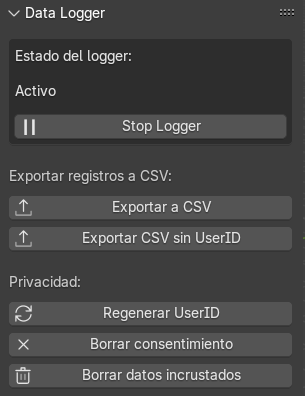
\includegraphics[width=0.78\textwidth, height=0.58\textheight, keepaspectratio]{diagramas/activo1.png}
\caption{Interfaz principal del \textit{add-on} de captura de datos.}
\label{fig:data_logger_sin_debug}
\end{figure}

\subsection{Datos registrados}

El CSV generado por el complemento agrupa información temporal, espacial, topológica y operacional. Cada fila representa un cambio relevante detectado durante la sesión, mientras que cada columna almacena una variable concreta utilizada posteriormente por el módulo de análisis. Esta estructura permite reconstruir la evolución temporal de la sesión, calcular métricas y comparar diferentes registros de modelado.

Los datos temporales permiten ordenar los eventos y medir la duración del proceso. Los datos espaciales describen la posición de la vista y del objeto activo. Los datos topológicos reflejan variaciones en la geometría de la malla. Por último, los campos operacionales identifican acciones relevantes del flujo de modelado, como duplicaciones, fusiones, cambios de modo o modificaciones UV.

\begin{table}[H]
\centering
\small
\begin{tabularx}{\textwidth}{p{0.24\textwidth}X}
\toprule
\textbf{Grupo de datos} & \textbf{Campos representativos} \\
\midrule
Metadatos & \texttt{SchemaVersion}, \texttt{LoggerVersion}, \texttt{SessionID}, \texttt{UserID}. \\
Temporales & \texttt{TimeStamp}, \texttt{Minute}, \texttt{Second}. \\
Vista y escena & \texttt{UserX}, \texttt{UserY}, \texttt{UserZ}, \texttt{SceneRadius}. \\
Objeto activo & \texttt{ObjX}, \texttt{ObjY}, \texttt{ObjZ}, \texttt{ObjRadius}, \texttt{ObjDeltaX}, \texttt{ObjDeltaY}, \texttt{ObjDeltaZ}, \texttt{ObjDeltaRadius}. \\
Topología & \texttt{VertexDelta}, \texttt{NgonDelta}, \texttt{TriDelta}, \texttt{NormalDelta}. \\
Estado y modo & \texttt{ObjModeState}, \texttt{EditModeState}, \texttt{ModeChanged}. \\
Operadores & \texttt{CtrlV}, \texttt{ShiftD}, \texttt{AltD}, \texttt{Merge}, \texttt{UV}. \\
Escena & \texttt{ObjectDelta}, \texttt{ModifierDelta}, \texttt{Occlusion}. \\
\bottomrule
\end{tabularx}
\caption{Agrupación resumida de los campos registrados por el \textit{Data Logger 3D}.}
\label{tab:campos_csv_resumen}
\end{table}

\subsection{Detección de cambios y persistencia}

La detección de operaciones se apoya en la observación del estado de la escena y en la identificación de operadores ejecutados por el usuario. Esta combinación permite registrar tanto cambios visibles en la geometría como acciones que no siempre producen una variación inmediata en el número de vértices o caras~\cite{blenderapi}.

El sistema también incorpora mecanismos de consentimiento, exportación anonimizada y borrado de datos. Los registros se escriben inicialmente en un CSV temporal y pueden quedar incrustados en el archivo \texttt{.blend} como bloque de texto interno, lo que facilita conservar la información junto al proyecto de modelado y exportarla posteriormente.

\section{Segundo \textit{add-on}: análisis y visualización}

El segundo complemento constituye la capa de explotación analítica. Su función es cargar los CSV generados por el \textit{Data Logger 3D}, validar su contenido, calcular métricas y presentar resultados comprensibles. El análisis puede aplicarse a un archivo individual o a un conjunto de registros, lo que permite comparar sesiones o estudiar distintos usuarios.

La lectura del CSV incluye comprobaciones de consistencia para evitar que valores incompletos, no numéricos o no finitos alteren los resultados. Esta validación es importante porque las métricas calculadas dependen directamente de la calidad de los datos registrados~\cite{mckinney2022python}.

La Figura~\ref{fig:add-on_analisis} presenta el panel principal del complemento de análisis.

\begin{figure}[H]
    \centering
    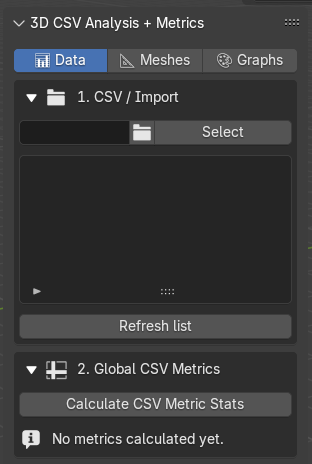
\includegraphics[width=0.42\textwidth]{diagramas/activo2.png}
    \caption{Panel principal del \textit{add-on} de análisis dentro de Blender.}
    \label{fig:add-on_analisis}
\end{figure}

\section{Flujo completo de análisis de datos}

El flujo completo comienza con la interacción del usuario durante el modelado. El complemento de captura observa la escena, detecta cambios relevantes y almacena los registros en formato CSV. Posteriormente, el complemento de análisis carga estos archivos, calcula métricas descriptivas, obtiene indicadores geométricos del modelo y genera visualizaciones integradas.

La Figura~\ref{fig:pipeline_analisis} resume el proceso completo.

\begin{figure}[H]
    \centering
    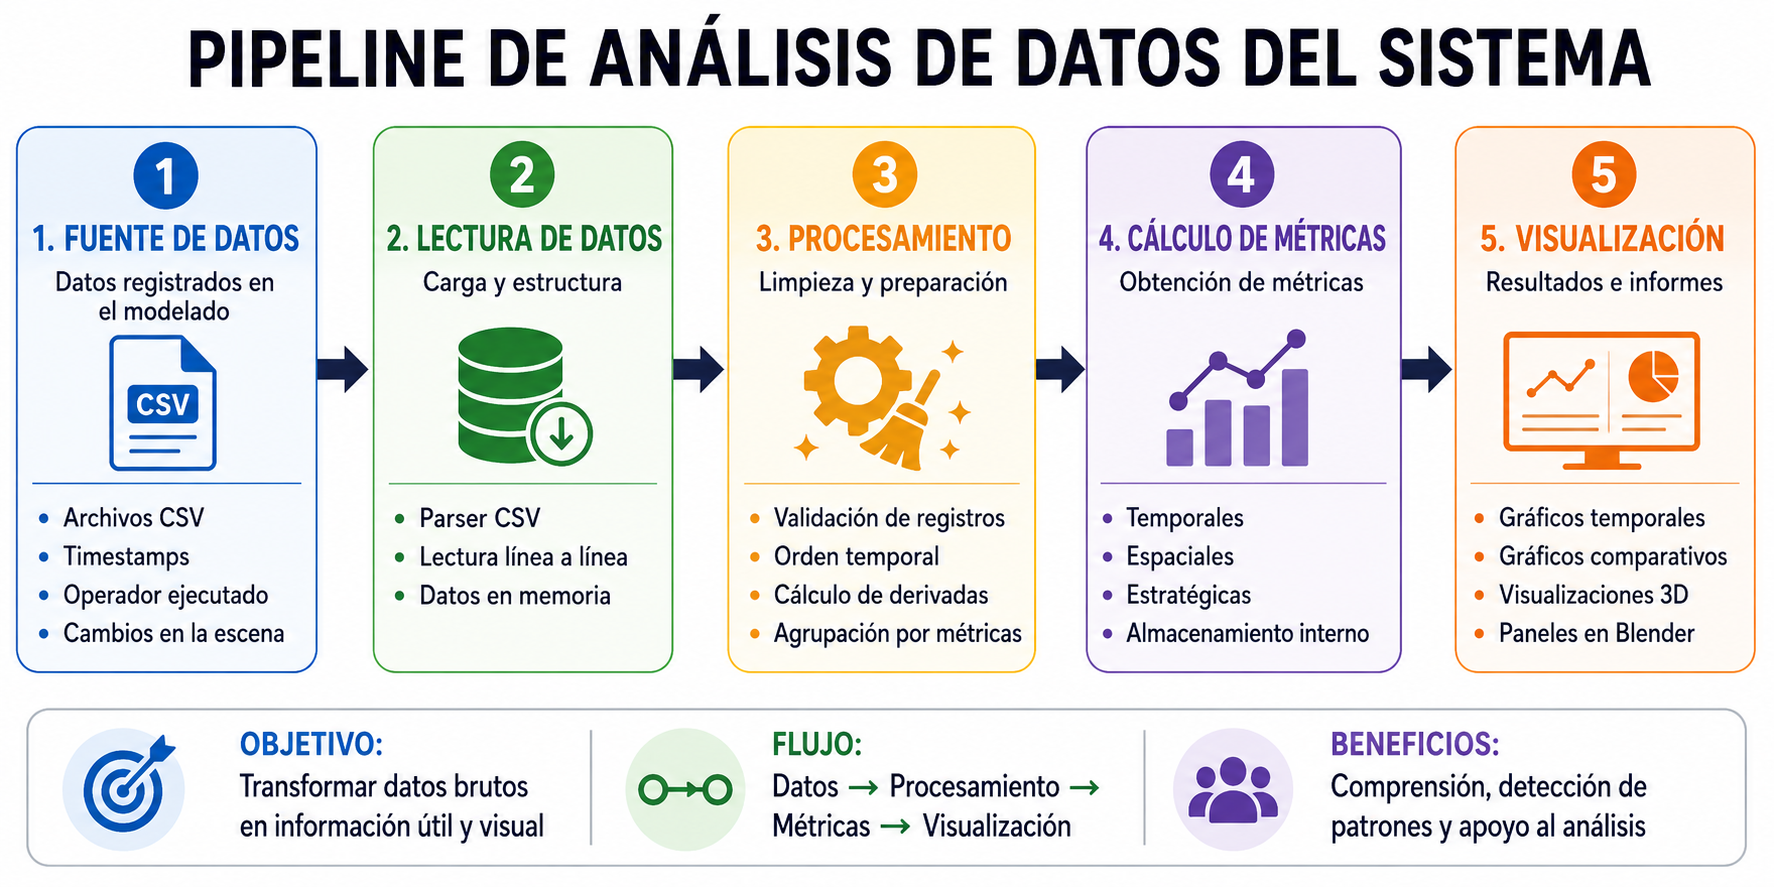
\includegraphics[width=0.9\textwidth]{diagramas/pipeline2.png}
    \caption{Pipeline general de captura, análisis y visualización de datos.}
    \label{fig:pipeline_analisis}
    {\footnotesize \textit{Nota. Figura elaborada por la autora con asistencia de ChatGPT.}}
\end{figure}

La separación entre captura y análisis evita sobrecargar la sesión de modelado. Durante la captura, la prioridad es registrar cambios sin interferir en el trabajo del usuario. En cambio, los cálculos estadísticos y geométricos pueden ejecutarse posteriormente, cuando el registro ya ha sido generado.

\section{Implementación del cálculo de métricas}

Las métricas descritas desde el punto de vista teórico en el Capítulo 3 se implementan en el segundo \textit{add-on} a partir de los registros CSV generados por \textit{Data Logger 3D}.

El proceso de cálculo sigue una secuencia común. En primer lugar, el complemento carga el archivo CSV y normaliza su contenido. A continuación, valida que las columnas necesarias existan y que los valores numéricos sean finitos. Después, transforma las columnas temporales, espaciales, topológicas y operacionales en los indicadores A1--A16. Finalmente, los resultados se agrupan para su consulta en la interfaz y para la generación de visualizaciones.

\begin{table}[H]
\centering
\small
\begin{tabularx}{\textwidth}{p{0.25\textwidth}p{0.28\textwidth}X}
\toprule
\textbf{Bloque de implementación} & \textbf{Datos de entrada} & \textbf{Resultado generado} \\
\midrule
Métricas temporales & \texttt{TimeStamp}, \texttt{Minute}, \texttt{Second} & Duración, pausas, distribución temporal y ritmo de actividad. \\
Métricas espaciales & \texttt{UserX}, \texttt{UserY}, \texttt{UserZ}, \texttt{ObjX}, \texttt{ObjY}, \texttt{ObjZ} & Velocidad de navegación, proximidad y picos de movimiento. \\
Métricas geométricas del CSV & \texttt{VertexDelta}, \texttt{NgonDelta}, \texttt{TriDelta}, \texttt{NormalDelta} & Indicadores de evolución estructural de la malla durante la sesión. \\
Métricas operacionales & \texttt{CtrlV}, \texttt{ShiftD}, \texttt{AltD}, \texttt{Merge}, \texttt{ModifierDelta}, \texttt{UV} & Indicadores de estrategia de edición y uso de operaciones relevantes. \\
Métricas sobre malla activa & Geometría evaluada mediante \texttt{Mesh}, \texttt{BMesh} y, cuando procede, \texttt{KDTree} & Área UV, islas UV, \textit{UV stretch}, densidad de texeles, normales, ángulos entre caras y similitud geométrica. \\
\bottomrule
\end{tabularx}
\caption{Implementación del cálculo de métricas a partir de los datos registrados y de la malla activa.}
\label{tab:implementacion_metricas}
\end{table}

Esta separación permite distinguir entre métricas derivadas del registro de sesión y métricas calculadas directamente sobre la geometría seleccionada. Las primeras describen la evolución temporal del proceso; las segundas analizan propiedades técnicas del modelo en el momento de la evaluación~\cite{cignoni1998metro,botsch2010polygon}.

\section{Cálculo geométrico y UV en el sistema}

Además del procesamiento del CSV, el complemento de análisis incorpora funciones que operan directamente sobre la malla activa. Estas funciones recorren vértices, caras, aristas y bucles UV para obtener información que no siempre aparece de forma explícita en el registro temporal.

Para estas operaciones se emplea \texttt{bmesh} cuando es necesario acceder a la geometría editable y \texttt{Mesh} cuando basta con consultar la malla evaluada. En el cálculo de similitud se utilizan distancias espaciales entre conjuntos de vértices y, cuando está disponible, una estructura \texttt{KDTree} para reducir el coste de búsqueda de vecinos cercanos. Esta parte del sistema permite complementar las métricas de sesión con indicadores técnicos del estado del modelo~\cite{bentley1975kdtree,blenderapi}.

\section{Generación de visualizaciones}

El sistema genera visualizaciones estadísticas y representaciones tridimensionales integradas en la escena. Para ello se combinan bibliotecas de análisis, como \textit{Matplotlib}~\cite{matplotlib}, con la creación procedural de mallas y materiales dentro de Blender. Esta integración permite presentar resultados analíticos en el propio contexto espacial del modelo~\cite{munzner2014visualization}.

La Figura~\ref{fig:radar_experto_novato} muestra un ejemplo de visualización tipo radar generada en el \textit{viewport}.

\begin{figure}[H]
    \centering
    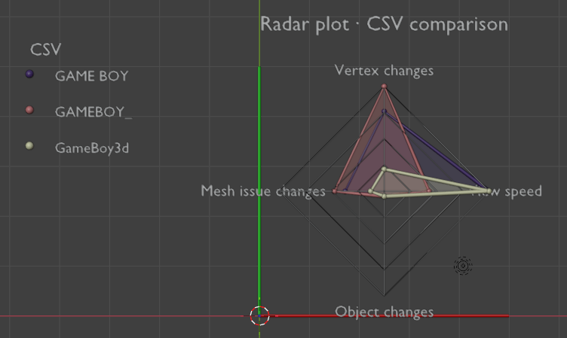
\includegraphics[width=0.86\textwidth]{diagramas/graficor1.png}
    \caption{Ejemplo de comparación de métricas mediante visualización de radar en el \textit{viewport}.}
    \label{fig:radar_experto_novato}
\end{figure}

\section{Decisiones técnicas relevantes}

Durante el desarrollo se adoptaron decisiones orientadas a mejorar la estabilidad, portabilidad y mantenibilidad del sistema~\cite{pressman2005}. La Tabla~\ref{tab:decisiones_tecnicas} resume las más relevantes.

\begin{table}[H]
\centering
\small
\begin{tabularx}{\textwidth}{p{0.28\textwidth}X}
\toprule
\textbf{Decisión} & \textbf{Justificación} \\
\midrule
Dos \textit{add-ons} independientes & Separar la adquisición de datos del procesamiento analítico. \\
CSV como formato intermedio & Facilitar la portabilidad, depuración y reutilización externa. \\
Captura basada en cambios & Reducir escrituras innecesarias y tamaño de los registros. \\
Detección de operadores & Registrar acciones relevantes que no siempre se reflejan directamente en la geometría. \\
\texttt{bmesh} & Acceder con mayor control a la geometría editable y a la información UV. \\
Validación previa al análisis & Evitar resultados alterados por datos incompletos, duplicados o no finitos. \\
\bottomrule
\end{tabularx}
\caption{Principales decisiones técnicas adoptadas durante el desarrollo.}
\label{tab:decisiones_tecnicas}
\end{table}

\section{Problemas encontrados y soluciones}

Durante el desarrollo se identificaron problemas relacionados con la captura de eventos, la interpretación de cambios en la malla, el tamaño del CSV y la legibilidad de los resultados. La Tabla~\ref{tab:problemas_soluciones} resume las principales incidencias y las soluciones aplicadas.

\begin{table}[H]
\centering
\small
\begin{tabularx}{\textwidth}{p{0.32\textwidth}X}
\toprule
\textbf{Problema} & \textbf{Solución aplicada} \\
\midrule
Diferencias entre \textit{Object Mode} y \textit{Edit Mode} & Uso combinado de \texttt{Mesh} y \texttt{BMesh} según el contexto activo. \\
Eventos no reflejados directamente en la geometría & Detección de operadores mediante la pila del \textit{WindowManager} y banderas binarias. \\
Cambios UV difíciles de identificar & Combinación de operadores UV conocidos y firma global de coordenadas. \\
Crecimiento excesivo del CSV & Captura diferencial y eliminación de filas duplicadas. \\
Datos inconsistentes en el análisis & Validación de campos, normalización del esquema y descarte de valores no finitos. \\
Dificultad de interpretación de resultados & Agrupación de métricas y generación de visualizaciones complementarias. \\
\bottomrule
\end{tabularx}
\caption{Problemas encontrados durante el desarrollo y soluciones adoptadas.}
\label{tab:problemas_soluciones}
\end{table}

\section{Validación y recogida de datos}

La validación del sistema se realizó mediante pruebas funcionales en Blender y mediante su utilización en una actividad práctica desarrollada en la Escuela de Arte y Superior de Diseño de Burgos. El objetivo fue comprobar el funcionamiento del flujo completo: activación del complemento, inicio de la captura, registro de operaciones de modelado, generación de CSV y posterior análisis de los datos.

Durante la actividad se realizaron sesiones de prueba con usuarios trabajando en Blender. El sistema permitió generar registros compatibles con el módulo de análisis y comprobar la viabilidad técnica del procedimiento en un contexto real de uso.

La Figura~\ref{fig:easd_actividad} documenta la actividad práctica realizada.

\begin{figure}[H]
\centering
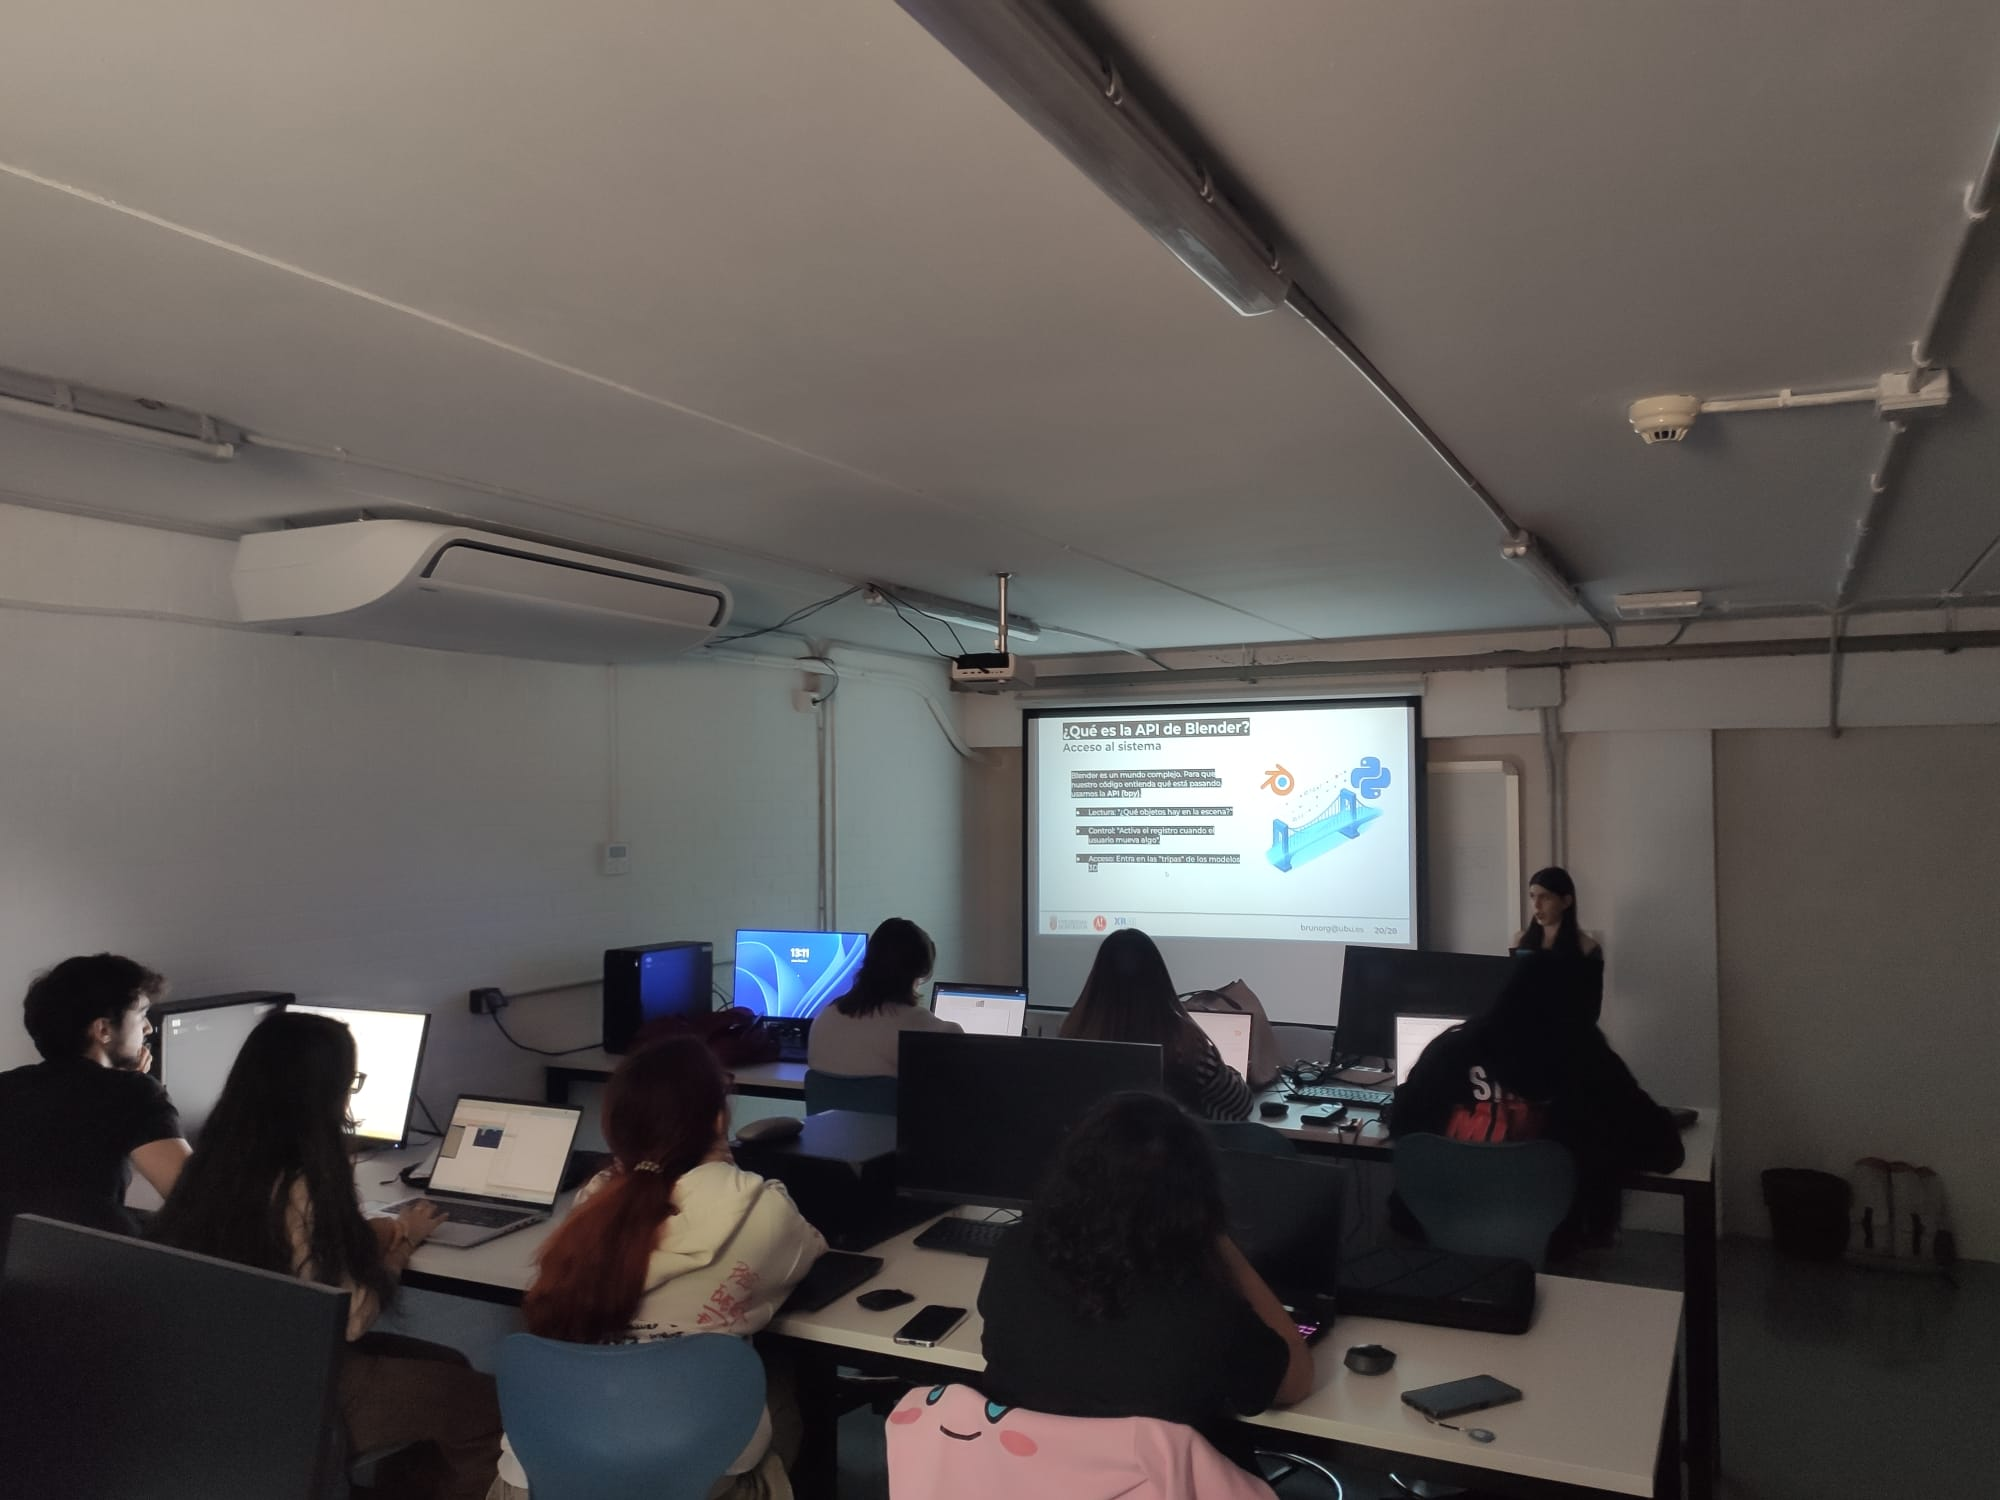
\includegraphics[width=0.85\textwidth]{diagramas/easd_actividad.png}
\caption{Actividad práctica realizada en la Escuela de Arte y Superior de Diseño de Burgos.}
\label{fig:easd_actividad}
\end{figure}

La validación debe entenderse como una prueba funcional en contexto real, no como un estudio estadístico con muestra representativa. Su finalidad fue comprobar la estabilidad básica de la captura, la correcta generación de los archivos CSV, la compatibilidad con el complemento de análisis y la detección de problemas prácticos de uso.

Durante esta fase se observó que algunos participantes no iniciaron correctamente el sistema de registro, por lo que no se pudieron recoger los datos de esas sesiones. Esta incidencia permitió identificar una limitación de usabilidad en el proceso de arranque y motivó la necesidad de reforzar las indicaciones de uso, los mensajes de estado y la documentación del procedimiento de inicio~\cite{nielsen1994usability}.

\subsection{Trazabilidad entre objetivos, implementación y validación}

Para relacionar los objetivos planteados con los componentes desarrollados y las evidencias de validación, se presenta la Tabla~\ref{tab:trazabilidad-objetivos}. Esta trazabilidad permite comprobar que las funcionalidades principales del sistema han sido implementadas y revisadas mediante pruebas funcionales o automatizadas.

\begin{table}[H]
\centering
\small
\begin{tabularx}{\textwidth}{p{0.20\textwidth}p{0.25\textwidth}p{0.25\textwidth}X}
\toprule
\textbf{Objetivo} & \textbf{Implementación} & \textbf{Validación} & \textbf{Evidencia} \\
\midrule
Registrar eventos de modelado &
\textit{Data Logger 3D}, handlers y temporizador &
Pruebas funcionales en Blender &
CSV de prueba y checklist de validación \\

Analizar sesiones registradas &
\textit{Analysis 3D} y módulos de análisis &
Pruebas de cálculo de métricas &
Resultados de métricas y pruebas del módulo \\

Mantener compatibilidad CSV &
Normalización de esquema y lectura validada &
Pruebas de carga de archivos &
CSV v1/v2 y validaciones de lectura \\

Proteger la privacidad &
UUID, exportación anonimizada y borrado de datos &
Revisión funcional &
CSV anonimizado y opciones de limpieza \\

Visualizar resultados &
Módulos de gráficos, escena y UI &
Prueba funcional dentro de Blender &
Capturas y visualizaciones generadas \\
\bottomrule
\end{tabularx}
\caption{Trazabilidad entre objetivos, implementación y validación.}
\label{tab:trazabilidad-objetivos}
\end{table}

\section{Reproducibilidad y material de entrega}

La entrega del proyecto incluye el código fuente de los dos complementos, instrucciones de instalación y uso, licencia del software, documentación asociada y material de validación~\cite{fsf_gpl3}. 

\section{Síntesis del desarrollo}

El desarrollo realizado demuestra la viabilidad de construir una herramienta modular para registrar y analizar procesos de modelado 3D. El primer complemento proporciona una base de captura no intrusiva y persistencia estructurada. El segundo transforma los registros en métricas interpretables y visualizaciones integradas. En conjunto, la solución permite estudiar sesiones de modelado, comparar registros y apoyar el análisis de procesos de aprendizaje en entornos tridimensionales.
